\SourcePage{739}{742}
\section{Behavior of Cross Sections Near a Reaction Threshold}

If the sum of the internal energies of the reaction products exceeds that of the initial particles, the reaction has a \emph{threshold}: it can occur only when the kinetic energy $E$ of the colliding particles (in the center-of-mass system) exceeds a definite threshold value $E_{\mathrm{th}}$. We shall examine the energy dependence of the reaction cross section near its threshold. We assume that the reaction once again produces only two particles (a reaction of the type $A+B=A'+B'$).

Near the threshold, the relative velocity $v'$ of the particles formed is small. This reaction is the reverse of one in which the velocity of the colliding particles is small. Its cross section as a function of $v'$ can therefore readily be found from the principle of detailed balance (144.13), using the known energy dependence of the reaction for which $v'$ would be

\SourcePage{740}{743}
the velocity in the entrance channel (\S~143). For a broad class of reactions in which there is no Coulomb interaction between $A'$ and $B'$ (for example, nuclear reactions producing a slow neutron), we thus find that the reaction cross section is proportional to $v'^2(1/v')$, that is,\footnote{The constancy of the limiting value approached by the amplitude $f_{fi}$ as $p_f\to0$, noted at the end of \S~144, corresponds precisely to this result: the cross section (144.4) is proportional to $p_f$.}
\begin{equation}
 \sigma_r\sim v'.
 \tag{147.1}
\end{equation}
This also gives the dependence of the cross section on the energy of the colliding particles: $v'$, and hence the reaction cross section, is proportional to the square root of $E-E_{\mathrm{th}}$:
\begin{equation}
 \sigma_r=A\sqrt{E-E_{\mathrm{th}}}.
 \tag{147.2}
\end{equation}

The scattering amplitudes in different channels are related by unitarity relations. Because of this connection, the opening of a new channel produces certain singular features in the energy dependence of the cross sections of other processes as well, including elastic scattering (E.~Wigner, 1948; A.~I.~Baz', 1957; G.~Breit, 1957). To determine the origin and character of this phenomenon, consider the simplest case, in which only elastic scattering is possible below the reaction threshold.

Near the threshold, the particles $A'$ and $B'$ are produced in a state with orbital angular momentum $l=0$ (this is precisely the state corresponding to the law (147.2)). If the particles taking part in the reaction have no spin, orbital angular momentum is conserved, and hence the $A+B$ system is also in an $s$ state. According to (142.7), the partial reaction cross section for $l=0$ is related to the $S$-matrix element for elastic scattering by
\begin{equation}
 \sigma_r=\frac\pi{k^2}(1-|S_0|^2),
 \tag{147.3}
\end{equation}
where $k$ is the wave vector of the colliding particles. Equating (147.2) and (147.3), we find that above and close to the reaction threshold, the modulus $|S_0|$, to terms of order $\sqrt{E-E_{\mathrm{th}}}$, is
\begin{equation}
 |S_0|=1-\frac{k_{\mathrm{th}}^2}{2\pi}A\sqrt{E-E_{\mathrm{th}}},\qquad E>E_{\mathrm{th}},
 \tag{147.4}
\end{equation}
where $k_{\mathrm{th}}=\sqrt{2mE_{\mathrm{th}}}/\hbar$ ($m$ is the reduced mass of particles $A$ and $B$). Below the threshold there is only elastic scattering, so
\begin{equation}
 |S_0|=1,\qquad E<E_{\mathrm{th}}.
 \tag{147.5}
\end{equation}

\SourcePage{741}{744}
But the scattering amplitude, and therefore $S_0$, must be analytic functions throughout the energy range. To the same accuracy, a function having the values (147.4) and (147.5) above and below the threshold is
\begin{equation}
 S_0=e^{2i\delta_0}\left(1-\frac{k_{\mathrm{th}}^2}{2\pi}A\sqrt{E-E_{\mathrm{th}}}\right),
 \tag{147.6}
\end{equation}
where $\delta_0$ is a constant (when $E<E_{\mathrm{th}}$, the root $\sqrt{E-E_{\mathrm{th}}}$ becomes imaginary, and the modulus of the expression in parentheses differs from unity only by a quantity of higher order).

For every $l\ne0$, however, inelastic scattering is absent, so
\begin{equation}
 S_l=e^{2i\delta_l},\qquad l\ne0,
 \tag{147.7}
\end{equation}
and in the region near the threshold the phases $\delta_l$ are to be set equal to their values at $E=E_{\mathrm{th}}$\footnote{Since the functions $\delta_l(E)$ are real both for $E>E_{\mathrm{th}}$ and for $E<E_{\mathrm{th}}$, they are expanded in integral powers of the difference $E-E_{\mathrm{th}}$.}.

Substitution of the resulting $S_l$ in (142.2) gives the following expression for the scattering amplitude near the reaction threshold:
\begin{equation}
 f(\theta,E)=f_{\mathrm{th}}(\theta)-\frac{k_{\mathrm{th}}}{4\pi}A
 \sqrt{E-E_{\mathrm{th}}}\,e^{2i\delta_0},
 \tag{147.8}
\end{equation}
where $f_{\mathrm{th}}(\theta)$ is the scattering amplitude at $E=E_{\mathrm{th}}$. The differential scattering cross section is consequently
\[
 \frac{d\sigma}{d\mathit{o}}=
 \begin{cases}
 |f_{\mathrm{th}}(\theta)|^2+\dfrac{k_{\mathrm{th}}}{2\pi}A\sqrt{E-E_{\mathrm{th}}}
 \Im\{f_{\mathrm{th}}(\theta)e^{-2i\delta_0}\},&E>E_{\mathrm{th}},\\
 |f_{\mathrm{th}}(\theta)|^2-\dfrac{k_{\mathrm{th}}}{2\pi}A\sqrt{E_{\mathrm{th}}-E}
 \Re\{f_{\mathrm{th}}(\theta)e^{-2i\delta_0}\},&E<E_{\mathrm{th}}.
 \end{cases}
\]
Writing the amplitude $f_{\mathrm{th}}$ as $|f_{\mathrm{th}}|e^{i\alpha(\theta)}$, we finally put this result in the form
\begin{equation}
 \frac{d\sigma}{d\mathit{o}}=|f_{\mathrm{th}}(\theta)|^2-
 \frac{k_{\mathrm{th}}}{2\pi}A|f_{\mathrm{th}}(\theta)|\sqrt{|E-E_{\mathrm{th}}|}
 \begin{cases}
 \sin(2\delta_0-\alpha),&E>E_{\mathrm{th}},\\
 \cos(2\delta_0-\alpha),&E<E_{\mathrm{th}}.
 \end{cases}
 \tag{147.9}
\end{equation}

According as the angle $2\delta_0-\alpha$ lies in the first, second, third, or fourth quadrant, the energy dependence of the cross section described by this formula has the form shown in Fig.~50a, b, c, or d. In every case there are two branches lying on opposite sides of a common vertical tangent.

When (147.9) is integrated over $d\mathit{o}$, only the isotropic part of the amplitude $f_{\mathrm{th}}(\theta)$---the partial amplitude for elastic

\SourcePage{742}{745}
$s$-wave scattering, $(e^{2i\delta_0}-1)/(2ik_{\mathrm{th}})$---makes a nonzero contribution to the integrals of the second terms. The total elastic-scattering cross section near the threshold is therefore
\begin{equation}
 \sigma=\sigma_{\mathrm{th}}-2A\sqrt{|E-E_{\mathrm{th}}|}
 \begin{cases}
 \sin^2\delta_0,&E>E_{\mathrm{th}},\\
 \sin\delta_0\cos\delta_0,&E<E_{\mathrm{th}}.
 \end{cases}
 \tag{147.10}
\end{equation}
This dependence has form a or b in Fig.~50 according as $\sin\delta_0\cos\delta_0$ is positive or negative.

Thus, the existence of a reaction threshold produces a characteristic feature in the energy dependence of the elastic-scattering cross section. Particle spin naturally changes the quantitative formulas, but the general character of the phenomenon remains the same\footnote{When the spins are nonzero, the $A'+B'$ system in an $s$ state may have nonzero total angular momentum, making different orbital states of the $A+B$ system possible.}. If reactions other than elastic scattering are also possible below the threshold, analogous features appear in their cross sections as well. At $E=E_{\mathrm{th}}$ all of them have a singularity near which they are linear functions of $\sqrt{|E-E_{\mathrm{th}}|}$, with different slopes above and below the threshold.

\begin{figure}[tbp]
\centering
\begin{tikzpicture}[x=0.72cm,y=0.50cm,line cap=round,line join=round]
\foreach \yy/\lab/\m/\k/\sleft/\sright in {12/{a}/1.25/.633/-1/-1,8/{b}/.7/.4/1/-1,4/{c}/.35/.45/1/1,0/{d}/.7/.4/-1/1}{
  \draw[->] (0,\yy) -- (5.4,\yy) node[right] {$E$};
  \draw[->] (0,\yy-1.15) -- (0,\yy+1.55) node[above] {$\dfrac{d\sigma}{dE}$};
  \draw[dashed] (2.7,\yy-1.0) -- (2.7,\yy+1.35);
  \draw[smooth,samples=60,domain=.35:2.7] plot (\x,{\yy+\m+\sleft*\k*sqrt(2.7-\x)});
  \draw[smooth,samples=60,domain=2.7:5.05] plot (\x,{\yy+\m+\sright*\k*sqrt(\x-2.7)});
  \node at (2.7,\yy-1.35) {\lab};
}
\end{tikzpicture}
\caption{}
\end{figure}

In nuclear reactions that emit a positively charged particle, there are Coulomb repulsive forces between the reaction products $A'$ and $B'$. In this case, as $v'\to0$ (that is, $E\to E_{\mathrm{th}}$), the reaction cross section tends exponentially to zero together with all its energy derivatives, and no singular feature arises in the cross sections of other processes.

Finally, consider reactions producing two oppositely charged slow particles, between which Coulomb attraction acts. By detailed balance, the cross section of such a reaction is related to the cross section (143.6) of the reverse reaction between two slow particles that attract one another. We thus find that as $v'\to0$ the cross section tends to a constant limit:
\begin{equation}
 \sigma_r=\mathrm{const}\quad\text{as }v'\to0,
 \tag{147.11}
\end{equation}
that is, beyond the threshold the reaction appears immediately with a finite cross section.

\SourcePage{743}{746}
Let us determine the character of the feature in the elastic-scattering cross section near the threshold of such a reaction (A.~I.~Baz', 1959). This cannot, however, be done directly from the known above-threshold law (147.11) by the simple method used above for uncharged particles. Compared with the latter case, the situation is now complicated by the fact that in the near-threshold region ($E<E_{\mathrm{th}}$), the $A'+B'$ system has bound states corresponding to discrete energy levels in the attractive Coulomb field. From an energy standpoint, these states can be formed in collisions of $A$ and $B$, but because elastic scattering is possible, they are only quasistationary. Their existence must nevertheless produce resonance effects in the below-threshold elastic scattering, analogous to Breit--Wigner resonances.

To solve the problem, consider the structure of the wave functions describing the collision process. Because there are two channels, the Schrödinger equation for the system of interacting particles has two independent solutions finite throughout configuration space; denote two arbitrarily chosen (and arbitrarily normalized) solutions by $\psi_1$ and $\psi_2$. Linear combinations describing scattering when either channel is the entrance channel can be formed from these functions. Denote the channels corresponding to the particle pairs $A,B$ and $A',B'$ by $a$ and $b$, and let the sum $\psi=a_1\psi_1+a_2\psi_2$ correspond to entrance channel $a$; it describes elastic scattering of $A$ and $B$ and the reaction $A+B\to A'+B'$. Near the reaction threshold, the coefficients $a_1,a_2$ depend essentially on the small momentum $k_b$, while the arbitrarily selected functions $\psi_1,\psi_2$ themselves have no singularity at $k_b=0$.

At large distances, $\psi$ must be a sum of two terms corresponding to the motion of the particle pairs in channels $a$ and $b$. Each is a product of the particles' ``internal'' functions and the wave function of their relative motion\footnote{The law (147.11) holds not only for the total cross section but also for partial cross sections with different angular momenta $l$ (cf. the end of \S~143). Thus, the singularity considered below also occurs in every partial scattering cross section. Its character is already fully revealed for $l=0$, which is the case examined below. The index 0 on the corresponding partial amplitudes is omitted to simplify the notation.}. In channel $a$, the latter has the form $R_a^- -S_{aa}R_a^+$, and in channel $b$ it is $-S_{ab}R_b^+$, where $R^+,R^-$ are the outgoing and incoming waves in the corresponding channels. At distances $r_0$ that are large

\SourcePage{744}{747}
compared with the range of the short-range forces and small compared with $1/k_b$, these functions (and their derivatives) must be ``matched'' to the values calculated from $\psi$ in the ``reaction zone.'' These conditions are expressed by equalities of the form
\[
 a_1\alpha_1+a_2\alpha_2=(R_a^--S_{aa}R_a^+)|_{r_0},\qquad
 a_1\beta_1+a_2\beta_2=-S_{ab}R_b^+|_{r_0},
\]
where $\alpha_1,\alpha_2,\beta_1,\beta_2,\ldots$ are quantities calculated from $\psi_1$ and $\psi_2$; by the preceding argument, near the threshold they may be regarded as constants independent of $k_b$. Dividing the first and second pairs of these equalities term by term, we obtain a system of two linear equations for two unknowns ($a_1/a_2$ and $S_{aa}$). Only one quantity that depends ``critically'' on $k_b$ occurs in the coefficients of these equations: the logarithmic derivative of the outgoing wave in channel $b$. Define it by
\[
 \Lambda=\left.\frac1{2\pi}\frac{(rR_b^+)'}{rR_b^+}\right|_{r=r_0}.
\]
There is no need actually to solve these equations. It is enough to observe that the quantity of interest, $S_{aa}$ (which determines the elastic-scattering amplitude), is a linear-fractional function of $\Lambda$. Below the threshold, $\Lambda$ is real because $R_b^+$ is real: it is a solution of a real Schrödinger equation with a real condition at infinity (decay as $e^{-\varkappa_b r}$, where $\varkappa_b=\sqrt{2m_b(E_{\mathrm{th}}-E)}/\hbar$). At the same time, below the threshold $|S_{aa}|=1$. It follows that the linear-fractional function $S_{aa}(\Lambda)$ must have the form
\begin{equation}
 S_{aa}=\frac{1+\beta\Lambda}{1+\beta^*\Lambda}e^{2i\eta},
 \tag{147.12}
\end{equation}
where $\eta$ is real and $\beta$ is a complex constant.

We now determine $\Lambda$ as a function of the momentum $k_b$. Since the particles $A'$ and $B'$ are subject to Coulomb attraction, $rR_b^+$ is given by the Coulomb wave function that is asymptotically proportional to $e^{ik_br}$ at infinity. In a repulsive Coulomb field this function is given by the sum $G_0+iF_0$, with $G_0$ and $F_0$ from (138.4) and (138.7). The transition to an attractive field is made by changing the signs of $k$ and $r$ simultaneously\footnote{Below we use Coulomb units. Changing the signs of $k$ and $r$ corresponds formally to changing the sign of the Coulomb unit of length.}. Making this

\SourcePage{745}{748}
substitution and calculating the logarithmic derivative (see \S~138), we obtain\footnote{To simplify the subsequent formulas, a real constant independent of $k_b$ ($-\ln2r_0-2C$) has been omitted from the braces. This amounts only to an inessential redefinition of the complex quantity $\beta$ and the real quantity $\eta$ in (147.12).}
\begin{equation}
 \Lambda=\frac{i}{1-\exp(-2\pi/k_b)}-\frac1\pi
 \left\{\ln k_b+\frac12\left[\psi\left(\frac{i}{k_b}\right)+
 \psi\left(-\frac{i}{k_b}\right)\right]\right\}.
 \tag{147.13}
\end{equation}
Here $k_b$ is assumed real, so this formula applies above the threshold. As $k_b\to0$, the first term in (147.13) tends to $i$, while the second tends to zero (see the note on p.~695). Thus, above the threshold,
\begin{equation}
 \Lambda=i,\qquad E>E_{\mathrm{th}}.
 \tag{147.14}
\end{equation}
The region below the threshold is reached by replacing $k$ by $i\varkappa$. Then (147.13), as $\varkappa\to0$, gives\footnote{The first term in (147.13) gives $-(1/2)\cot(\pi/\varkappa_b)+i/2$, while the expression in braces becomes $(\pi/2)\cot(\pi/\varkappa_b)+i\pi/2$. Here we use $\psi(x)-\psi(-x)=-\pi\cot\pi x-1/x$ (obtainable by logarithmic differentiation of the known relation $\Gamma(x)\Gamma(-x)=-\pi/(x\sin\pi x)$) and the limiting expression $\psi(x)\approx\ln x-1/2x$ as $x\to\infty$.}
\begin{equation}
 \Lambda=\cot\frac\pi{\varkappa_b},\qquad E<E_{\mathrm{th}}.
 \tag{147.15}
\end{equation}

These formulas solve the problem. The elastic-scattering cross section is
\[
 \sigma_e=\frac\pi{k_a^2}|S_{aa}-1|^2.
\]
Above the threshold,
\begin{equation}
 S_{aa}=\frac{1+i\beta}{1+i\beta^*}e^{2i\eta},
 \tag{147.16}
\end{equation}
and, like the reaction cross section, the scattering cross section is constant in this region. Note that the condition $|S_{aa}|\leq1$ requires $\Im\beta>0$.

Below the threshold we find
\begin{equation}
 S_{aa}=e^{2i\eta}\frac{\beta-\tan(\pi/\varkappa_b)}
 {\beta^*-\tan(\pi/\varkappa_b)}.
 \tag{147.17}
\end{equation}
This expression has infinitely many resonances accumulating toward $E=E_{\mathrm{th}}$. The resonance energies are roots of $S_{aa}=-1$, that is,
\[
 \Re\left\{e^{i\eta}\left(\beta-\tan\frac\pi{\varkappa_b}\right)\right\}=0;
\]

\SourcePage{746}{749}
they are shifted from the pure Coulomb levels (the roots of $\tan(\pi/\varkappa_b)=0$) by the presence of the short-range forces. As $E$ approaches the threshold, the elastic-scattering cross section oscillates between zero and $4\pi/k_a^2$, as shown schematically in Fig.~51. The width of the entire below-threshold region in which the resonance structure appears is set by the energy of the first Coulomb level\footnote{We mention one more interesting case of a near-threshold reaction: ionization of an atom by an electron whose energy only slightly exceeds the atom's first ionization energy. Under these conditions the collision process can be treated semiclassically, but the presence of three charged particles in the final state makes the problem very complicated. A general solution of this difficult problem was given by Wannier (G.~H.~Wannier // Phys. Rev. 1953. V.~90. P.~817). The ionization probability of a neutral atom is proportional to $(E-I)^\alpha$, where $\alpha=(1/4)(\sqrt{9173}-1)\approx1{.}13$, and $E-I$ is the excess of the electron energy above the ionization threshold.}.

\begin{figure}[tbp]
\centering
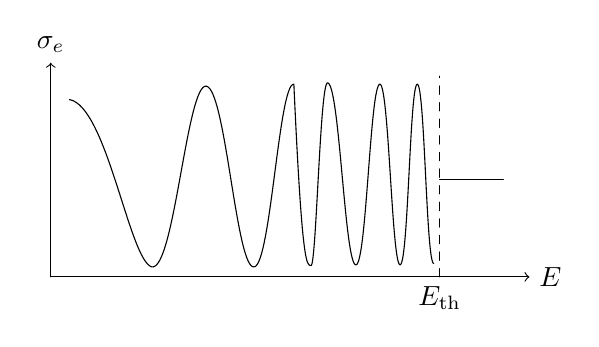
\begin{tikzpicture}[x=0.95cm,y=0.85cm,line cap=round,line join=round]
 \draw[->] (0,0) -- (6.4,0) node[right] {$E$};
 \draw[->] (0,0) -- (0,3.2) node[above] {$\sigma_e$};
 \draw[dashed] (5.2,0) -- (5.2,3.0);
 \node[below] at (5.2,0) {$E_{\mathrm{th}}$};
 \draw (0.25,2.65)
  .. controls (0.75,2.55) and (1.05,0.25) .. (1.35,0.15)
  .. controls (1.65,0.08) and (1.82,2.9) .. (2.08,2.85)
  .. controls (2.34,2.8) and (2.48,0.1) .. (2.72,0.15)
  .. controls (2.94,0.18) and (3.05,2.9) .. (3.25,2.88)
  .. controls (3.36,0.17) and (3.42,0.17) .. (3.48,0.17)
  .. controls (3.55,0.17) and (3.6,2.9) .. (3.7,2.9)
  .. controls (3.86,2.9) and (3.93,0.17) .. (4.08,0.18)
  .. controls (4.22,0.18) and (4.27,2.88) .. (4.4,2.88)
  .. controls (4.52,2.88) and (4.56,0.18) .. (4.67,0.18)
  .. controls (4.78,0.18) and (4.8,2.88) .. (4.9,2.88)
  .. controls (5.0,2.88) and (5.02,0.2) .. (5.12,0.2);
 \draw (5.2,1.45) -- (6.05,1.45);
\end{tikzpicture}
\caption{}
\end{figure}
